\documentclass{standalone}

\usepackage{tikz}
\usepackage{../../style/csmacros}

\definecolor{bleu1}{RGB}{38, 196, 236}
\definecolor{rouge1}{RGB}{231, 62, 1}
\definecolor{EdfBlue}{RGB}{0,112,192}
\definecolor{EdfDBlue}{RGB}{9,53,122}
\definecolor{EdfLBlue}{RGB}{56,174,255}
\definecolor{EdfOrange}{RGB}{254,88,21}
\definecolor{EdfLOrange}{RGB}{243,157,0}
\definecolor{EdfGreen}{RGB}{80,158,47}
\definecolor{EdfLGreen}{RGB}{196,214,47}
\definecolor{EdfGrey}{RGB}{127,127,127}

\begin{document}
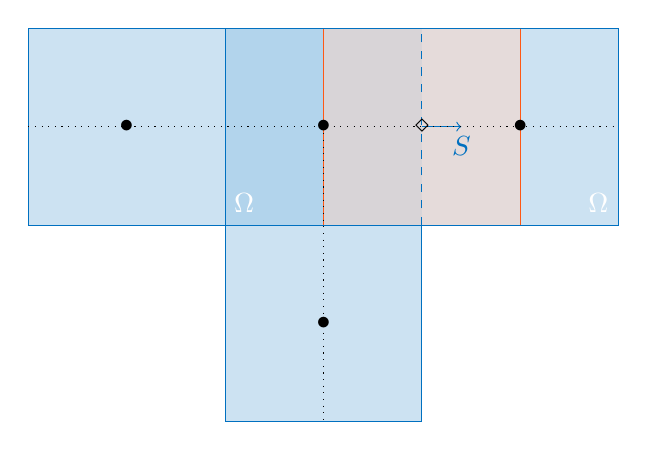
\begin{tikzpicture}[scale=2.5]
\fill[EdfBlue!20] (-1.0,0.0) rectangle (0.0,1.0);
\draw[EdfBlue] (-1.0,0.0) rectangle (0.0,1.0);
\fill[EdfBlue!20] (0.0,-1.0) rectangle (1.0,0.0);
\draw[EdfBlue] (0.0,-1.0) rectangle (1.0,0.0);
\fill[EdfBlue!30] (0.0,0.0) rectangle (1.0,1.0);
\fill[EdfBlue!20] (1.0,0.0) rectangle (2.0,1.0);
\fill[EdfOrange!25,opacity=0.5] (0.5,0.0) rectangle (1.5,1.0);
\draw[EdfOrange] (0.5,0.0) rectangle (1.5,1.0);
\draw[EdfBlue] (0.0,0.0) rectangle (2.0,1.0);
\draw[EdfBlue,dashed] (1.0,0.0) -- (1.0,1.0);
\draw[EdfBlue,->] (1.0,0.5) -- (1.2,0.5)node[below]{\textcolor{EdfBlue}{$\vect{S}_{\bij}$}};
\draw (0.5,0.5) node{\textcolor{black}{$\bullet$}};
\draw (0.5,0.5) node[below]{\textcolor{black}{$\celli$}};
\draw (1.5,0.5) node{\textcolor{black}{$\bullet$}};
\draw (1.5,0.5) node[below]{\textcolor{black}{$\cellj$}};
\draw (0.1,0.1) node{\textcolor{white}{$\Omega_{\celli}$}};
\draw (1.9,0.1) node{\textcolor{white}{$\Omega_{\cellj}$}};
\draw (-0.5,0.5) node{\textcolor{black}{$\bullet$}};
\draw (0.5,-0.5) node{\textcolor{black}{$\bullet$}};
\draw (1.0,0.5) node{\textcolor{black}{$\diamond$}};
\draw (1.0,0.5) node[below left]{\textcolor{black}{$\face$}};
\draw[dotted] (-1.0,0.5) -- (2.0,0.5);
\draw[dotted] (0.5,0.5) -- (0.5,-1.0);
\end{tikzpicture}
\end{document}
